\documentclass[10pt]{article}
\usepackage[margin=1in]{geometry}
\usepackage{times}
\usepackage[T1]{fontenc}
\usepackage{microtype}
\usepackage{amsmath,amssymb,amsthm}
\usepackage{booktabs}
\usepackage{graphicx}
\usepackage[numbers,sort&compress]{natbib}
\usepackage{xcolor}
\usepackage{tikz}
\usetikzlibrary{positioning,arrows.meta}
\usepackage[colorlinks=true,linkcolor=blue!50!black,citecolor=blue!50!black,urlcolor=blue!50!black]{hyperref}
\usepackage[capitalise,noabbrev]{cleveref}

\newtheorem{proposition}{Proposition}
\newcommand{\ztb}{\textsc{ZT-RAGBench}}
\newcommand{\pmci}[1]{{\scriptsize$\pm$#1}}

\title{Authorization Across the Enterprise RAG Request Lifecycle:\\An Empirical Zero-Trust Evaluation of Retrieval-Time and Release-Time Data Leakage}
\author{Naeem Shahzad\\
Riyadh, Saudi Arabia \quad ORCID: \href{https://orcid.org/0009-0003-2094-1553}{0009-0003-2094-1553}\\
% TODO: confirm affiliation (employer permission) and correspondence e-mail
}
\date{}

\begin{document}
\maketitle

\begin{abstract}
Enterprise retrieval-augmented generation (RAG) assistants answer questions over documents whose access rights differ by user and change over time. Most permission-aware designs settle authorisation once, when evidence is retrieved. We argue that authorisation is a property of the whole request lifecycle: ingestion, retrieval, caching, generation and release. We evaluate it at each stage with \ztb{}, a reproducible benchmark built on a synthetic multi-tenant corpus (6{,}000 documents, 18{,}000 chunks, attribute-based policies for 300 users). At the \emph{retrieval stage}, a shared index without access control exposes unauthorised content to 93.9\% of benign queries, and tenant partitioning still exposes 81.3\%. Post-retrieval filtering prevents exposure but costs 17--34 points of Hit@5. Query-time pre-filtering is optimal on a static corpus but leaks through stale access-control snapshots, derived artefacts and identity-agnostic semantic caches. At the \emph{release stage}, we formalise a commit-time invariant: every evidence dependency of a response must be authorised when the response is released. We measure how retrieval-only designs violate it when rights are revoked mid-request. With a 5-minute entitlement cache, each revocation of a departing insider is followed by 3.1 unsafe releases on average. Even live retrieval-time checks leave 0.64 unsafe releases per revocation for 60-second agentic tasks. A release-time recheck reduces this by 96\%, but neither recheck nor an atomic gate eliminates it while decisions are read from a lagging policy replica. Atomicity and freshness are \emph{jointly} required, and only a gate fenced against the authoritative policy store released zero unsafe responses, in both simulation and a multithreaded prototype (0 of $\sim$31{,}000 audited releases versus 12.3 unsafe releases per 100 revocations for a non-atomic recheck). We quantify the residual risks this gate leaves, namely streaming before the decision, incomplete provenance and policy-service outages, and derive deployment recommendations. Code, data generators and per-seed results are released.
\end{abstract}

\noindent\textbf{Keywords:} retrieval-augmented generation; zero-trust architecture; access control; authorization revocation; time-of-check to time-of-use; data leakage; enterprise AI.

\section{Introduction}
Retrieval-augmented generation (RAG)~\cite{lewis2020rag} gives language-model assistants access to organisational knowledge such as HR files, contracts, financial statements and engineering runbooks. Each source system enforces its own permissions. Indexing them into one retrieval store turns those permissions into metadata, and the RAG pipeline may or may not honour it. The OWASP Top~10 for LLM Applications now lists misaligned access control in vector stores, and context leakage between users who share them, as a distinct risk~\cite{owasp2025}.

Two lines of evidence make this risk concrete. First, content that reaches a model's context can be extracted. Structured prompts recover retrieval data verbatim~\cite{zeng2024good,qi2024spill}, indirect prompt injection redirects models through retrieved text~\cite{greshake2023}, and embeddings themselves can be inverted~\cite{morris2023}. Second, permission-aware RAG is an active research area. Recent systems filter retrieval through provider-native identity and access management (IAM)~\cite{jeong2025permission}, combine role, trust and privacy controls~\cite{saxena2026pppa}, or argue for deterministic enforcement across all participants of an interaction~\cite{bhatt2025participant}.

These systems mostly treat authorisation as a \emph{retrieval-time} decision. In practice, rights change continuously: people move departments, leave projects and resign, and entitlement caches, replicas and index snapshots lag behind the authoritative directory. A request may retrieve evidence legitimately and still release a response derived from it after the user's right to that evidence has been withdrawn. Agentic workflows that run for a minute or more make this window wide. Time-of-check to time-of-use (TOCTOU) problems in LLM agents~\cite{lilienthal2025toctou}, stale facts in agent memory~\cite{shen2026revoked} and revocation in delegated agent credentials~\cite{parakhin2026} show that the issue is real. However, no prior work has measured it for RAG release decisions or compared it with the better-known retrieval-time failure modes.

This paper treats authorisation as a property of the \emph{whole request lifecycle} and asks:
\begin{itemize}\itemsep0pt
\item \textbf{RQ1.} How much unauthorised content reaches the generator under common retrieval-stage architectures, and at what utility cost is it prevented?
\item \textbf{RQ2.} Which operational conditions (entitlement-sync lag, derived artefacts, shared caches, mislabelling) cause retrieval-stage controls that are correct in a static setting to leak?
\item \textbf{RQ3.} When rights are revoked while a request is in flight, how many responses are released that depend on revoked evidence, and how does this depend on entitlement caching, release-time rechecks, atomicity and policy freshness?
\item \textbf{RQ4.} What residual risk remains under a commit-time gate (streaming, provenance gaps, policy-service outages), and what do the controls cost?
\end{itemize}

\paragraph{Contributions.}
(1)~A lifecycle threat model and leakage metrics for enterprise RAG, including a \emph{commit-time evidence-authorisation invariant} with explicit consistency assumptions (\cref{sec:model}).
(2)~\ztb{}, an open benchmark with a multi-tenant corpus, attribute-based access control (ABAC)~\cite{nist800162}, ten experiments and five-seed confidence intervals (\cref{sec:method}).
(3)~Measurements of six retrieval-stage architectures under static and dynamic conditions (\cref{sec:resA}).
(4)~The first quantitative study of in-flight revocation in RAG release decisions. It shows that a release-time recheck is necessary but not sufficient, and that atomicity without policy freshness gives no measurable benefit. A multithreaded prototype confirms these results under real interleavings (\cref{sec:resB}).
(5)~A zero-trust reference pipeline and deployment recommendations grounded in the measurements (\cref{sec:discussion}).

\section{Background and Related Work}
\label{sec:related}
\paragraph{Attacks on RAG data.}
Zeng et al.~\cite{zeng2024good} pair a retrieval-steering prompt with an instruction to repeat the context, and show that RAG datastores leak under such composite prompts. Qi et al.~\cite{qi2024spill} extract datastore text verbatim from instruction-tuned models through prompt injection. Greshake et al.~\cite{greshake2023} introduced indirect prompt injection via retrieved content, PoisonedRAG~\cite{zou2025poisonedrag} corrupts the knowledge base, and Morris et al.~\cite{morris2023} invert embeddings to text. SafeRAG~\cite{liang2025saferag} benchmarks RAG components against manipulated knowledge (silver noise, inter-context conflict, soft advertising and denial-of-service). We take the defender's perspective and assume that anything in the context is extractable. We therefore measure whether unauthorised content \emph{reaches} the context or the released response at all.

\paragraph{Permission-aware RAG.}
Jeong and Lee~\cite{jeong2025permission} enforce resource-level access control in multi-resource RAG by querying provider-controlled IAM systems. Saxena et al.~\cite{saxena2026pppa} integrate role-based rules, trust computation and privacy protection in cloud RAG (PPPARITL). Bhatt et al.~\cite{bhatt2025participant} argue that enterprise AI must enforce access control deterministically for every participant in an interaction. A recent review by Alghamdi~\cite{alghamdi2026review} organises RAG security risks by pipeline stage and notes the lack of benchmarks for authorisation state. Our work is complementary. Rather than proposing another retrieval filter, we measure \emph{where and when} enforcement must happen, comparing common designs across the whole lifecycle.

\paragraph{Revocation and TOCTOU in LLM systems.}
Lilienthal and Hong~\cite{lilienthal2025toctou} present a study of TOCTOU vulnerabilities in LLM agents, in which checked external state changes before it is used. Shen et al.~\cite{shen2026revoked} show that agent-memory systems often return facts that were soft-revoked, and propose a read-time validity guard. Parakhin~\cite{parakhin2026} models credential revocation in multi-agent delegation as a cache-coherence problem. They bound unauthorised operations per capability by an operation budget rather than a time-to-live, and evaluate the bound in simulation. On the standards side, the OpenID Continuous Access Evaluation Profile (CAEP)~\cite{caep2025} lets identity providers push events such as session revocation to relying parties, so that they can re-evaluate access while a session is active. None of these works studies the specific race between a revocation and the \emph{release of a RAG response} whose evidence was retrieved under the old policy. Nor do they quantify how entitlement caching, rechecks, atomicity and replica freshness interact. That race is the focus of \cref{sec:resB}.

\paragraph{Access-control foundations.}
Complete mediation~\cite{saltzer1975} requires every access to be checked; lattice-based information flow~\cite{denning1976} labels combined information with the least upper bound of its sources; ABAC~\cite{nist800162} evaluates policy over subject, object and environment attributes. NIST SP~800-207~\cite{nist800207} defines zero-trust architecture around per-request decisions by a policy decision point (PDP) enforced at policy enforcement points (PEPs). SP~800-207A~\cite{nist800207a} extends this model to cloud-native, multi-location applications. Semantic caches such as GPTCache~\cite{bang2023gptcache} answer repeated questions from stored responses, usually keyed on query similarity alone. In Saudi Arabia, the Personal Data Protection Law~\cite{pdpl2023}, in force since 14 September 2023, turns leakage of personal records through an assistant into a compliance event.

\section{System Model, Threat Model and the Commit-Time Invariant}
\label{sec:model}
\paragraph{Policy.}
Each document $d$ has a tenant $t(d)$, a department $\mathrm{dept}(d)$, a sensitivity level $\ell(d)$ (\textsc{Internal}, \textsc{Confidential} or \textsc{Restricted}, abbreviated \textsc{I}, \textsc{C}, \textsc{R}) and, for \textsc{R} documents, a set of project groups $G(d)$. Users carry tenant, department, clearance and group attributes. The authoritative policy at time $\tau$ is
\begin{equation}
\begin{aligned}
\mathrm{Allow}(u,d,\tau) = [t(u)=t(d)] \wedge \big(\, & \ell(d)=\textsc{I}\\
\vee\; & (\ell(d)=\textsc{C} \wedge \mathrm{dept}_\tau(u)=\mathrm{dept}(d) \wedge \mathrm{clr}(u)\ge \textsc{C})\\
\vee\; & (\ell(d)=\textsc{R} \wedge G_\tau(u)\cap G(d)\neq\emptyset \wedge \mathrm{clr}(u)=\textsc{R})\,\big),
\end{aligned}
\end{equation}
where $\mathrm{dept}_\tau$ and $G_\tau$ are the user's attributes in the authoritative directory at $\tau$. A chunk $c$ has a source set $S(c)$, and derived artefacts such as summaries have $|S(c)|>1$. A chunk is authorised iff all of its sources are, which is the least-upper-bound rule~\cite{denning1976}.

\paragraph{Request lifecycle.}
A request by $u$ arriving at $\tau_0$ retrieves evidence in one or more rounds, generates a draft and releases the response at a \emph{commit} time $\tau_c$, after which it cannot be recalled. Its dependency set $\mathrm{Deps}(o)$ contains every document whose content could have influenced output $o$. This includes the sources of retrieved chunks, cached contexts and intermediate agent summaries.

\paragraph{Adversaries.}
\emph{(A1)~Curious insider:} targets a same-tenant document they may not read, using a distinctive term such as a project code or client identifier. \emph{(A2)~Cross-tenant prober:} the same, targeting another tenant's document. \emph{(A3)~Stale principal:} keeps querying after a revocation. \emph{(A4)~Cache co-user:} asks a question similar to one asked earlier by a more privileged colleague. \emph{(A5)~Departing insider:} expects to lose access soon (a transfer or resignation) and keeps requests in flight around the revocation. We also measure \emph{incidental} exposure of benign users. The policy authority and the retrieval infrastructure are trusted; knowledge poisoning~\cite{zou2025poisonedrag}, embedding inversion~\cite{morris2023} and side channels are out of scope.

\paragraph{Metrics.}
Because context contents are extractable~\cite{zeng2024good,qi2024spill}, retrieval-stage leakage is measured at the retriever--generator boundary:
\begin{itemize}\itemsep0pt
\item \textbf{Exposure rate (ER):} the share of queries whose context contains an unauthorised chunk.
\item \textbf{Attack success rate (ASR):} the share of targeted queries that retrieve the target.
\item \textbf{Hit@5:} the share of benign queries that retrieve the intended authorised document.
\item \textbf{Oracle overlap:} the overlap with the top-5 results over exactly the authorised chunks.
\end{itemize}
Release-stage leakage is measured per revocation event:
\begin{itemize}\itemsep0pt
\item \textbf{Unsafe releases per revocation:} responses committed after the revocation whose dependencies include a lost document.
\item \textbf{$P(\text{any unsafe})$:} the probability that a revocation is followed by at least one unsafe release.
\item \textbf{Exposure window:} the time from the revocation to the last unsafe commit.
\item \textbf{Leaked tokens:} for streaming, the tokens emitted after the revocation.
\end{itemize}
Costs are measured as added latency, policy-check volume and false blocks during policy-service outages.

\paragraph{The commit-time invariant.}
\emph{For every committed output $o$ released to $u$ at commit time $\tau_c$, $\forall d\in\mathrm{Deps}(o): \mathrm{Allow}(u,d,\tau_c)$; otherwise $o$ is not committed.} The invariant concerns new releases after a revocation takes effect. A response delivered before the revocation is not a violation, and tool side effects need their own controls. It holds under five assumptions:
\begin{itemize}\itemsep0pt
\item[(C1)] $\mathrm{Deps}(o)$ is complete.
\item[(C2)] Policy reads and policy writes are linearisable at the authority.
\item[(C3)] No part of $o$ is emitted before the commit decision.
\item[(C4)] The decision and the commit are ordered together with revocations.
\item[(C5)] The decision reads the authority itself, not a lagging replica.
\end{itemize}

\begin{proposition}
Under (C1)--(C5), a gate that evaluates $\mathrm{Allow}$ for all recorded dependencies and commits in the same critical section that serialises policy writes never commits an output that violates the invariant.
\end{proposition}
\begin{proof}[Proof sketch]
Suppose that $o$ is committed at $\tau_c$ and that some $d\in\mathrm{Deps}(o)$ was revoked at $\tau_r<\tau_c$. By (C2) and (C4), the revocation is ordered before the gate's critical section. By (C5), the gate observes it, and by (C1), $d$ is checked. The gate therefore aborts, contradicting the assumption that $o$ was committed. (C3) ensures that nothing escaped before the decision.
\end{proof}
The value of the proposition lies in its assumptions. \Cref{sec:resB} measures what happens when each one fails, which is the normal state of deployed systems.

\section{Architectures Compared}
\label{sec:arch}
\paragraph{Retrieval stage (A0--A5).}
\textbf{A0} uses one shared index with no access control; retrieval runs under a service identity. \textbf{A1} partitions the index by tenant. \textbf{A2} filters the top-$k$ results after retrieval. \textbf{A3} over-fetches $4k$ results and then filters. \textbf{A4} pushes the access predicate into the search (pre-filtering) using an index-time access-control snapshot, and derived chunks inherit their primary source's ACL. \textbf{A5} is a zero-trust pipeline (\cref{fig:zt}) with seven principles:
\begin{itemize}\itemsep0pt
\item[P1] End-to-end user identity.
\item[P2] A per-request PDP decision on live attributes.
\item[P3] Enforcement inside retrieval.
\item[P4] Most-restrictive labels for derived chunks.
\item[P5] Re-authorisation of cached contexts on every hit.
\item[P6] An ingestion-time label/content consistency check that quarantines \textsc{Internal}-labelled documents containing PII-like fields.
\item[P7] A fenced commit-time release gate.
\end{itemize}

\paragraph{Release stage (S0--S4).}
\textbf{S0} checks at retrieval only, with entitlements cached for a TTL (default 5\,min). \textbf{S1} checks at retrieval only, on live attributes read through a policy replica. \textbf{S2} is S1 plus a \emph{non-atomic} recheck after generation, followed by post-processing (output filters, citation rendering, serialisation) before the commit. \textbf{S3} is S1 plus an \emph{atomic} gate whose decision and commit are fused but read from the replica. \textbf{S4} is S1 plus a \emph{fenced} gate that validates dependencies against the authority in the same critical section as revocations, which is P7. For streaming responses we also evaluate \emph{re-authorisation leases}: the stream is checked against the authority every $\Lambda$ seconds and aborted on the first denial.

\begin{figure}[t]
\centering
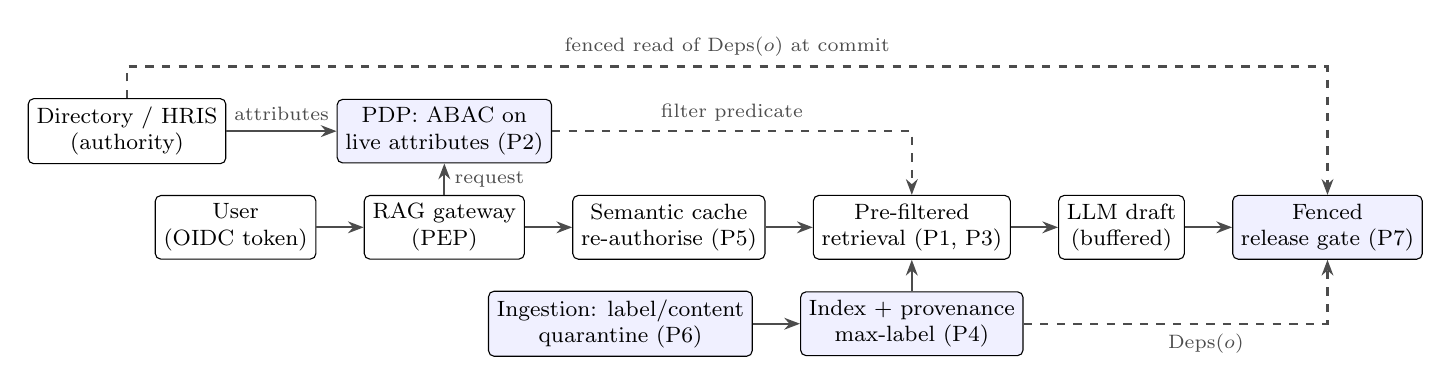
\begin{tikzpicture}[
  node distance=4mm and 6mm,
  box/.style={draw, rounded corners=2pt, align=center, font=\footnotesize, minimum height=8mm, inner sep=3pt, fill=white},
  pol/.style={box, fill=blue!6},
  arr/.style={-{Stealth[length=2mm]}, thick, draw=black!70},
  lbl/.style={font=\scriptsize, text=black!70}]
\node[box] (user) {User\\(OIDC token)};
\node[box, right=of user] (gw) {RAG gateway\\(PEP)};
\node[pol, above=of gw] (pdp) {PDP: ABAC on\\live attributes (P2)};
\node[box, left=14mm of pdp] (idp) {Directory / HRIS\\(authority)};
\node[box, right=of gw] (cache) {Semantic cache\\re-authorise (P5)};
\node[box, right=of cache] (ret) {Pre-filtered\\retrieval (P1, P3)};
\node[box, right=of ret] (llm) {LLM draft\\(buffered)};
\node[pol, right=of llm] (gate) {Fenced\\release gate (P7)};
\node[pol, below=of ret] (idx) {Index + provenance\\max-label (P4)};
\node[pol, left=of idx] (ing) {Ingestion: label/content\\quarantine (P6)};
\draw[arr] (user) -- (gw);
\draw[arr] (gw) -- (cache);
\draw[arr] (cache) -- (ret);
\draw[arr] (ret) -- (llm);
\draw[arr] (llm) -- (gate);
\draw[arr] (gw) -- node[lbl, right]{request} (pdp);
\draw[arr] (idp) -- node[lbl, above]{attributes} (pdp);
\draw[arr] (ing) -- (idx);
\draw[arr] (idx) -- (ret);
\draw[arr, dashed] (pdp.east) -| node[lbl, above, pos=0.25]{filter predicate} (ret.north);
\draw[arr, dashed] (idp.north) |- ++(0,4mm) -| node[lbl, above, pos=0.25]{fenced read of Deps$(o)$ at commit} (gate.north);
\draw[arr, dashed] (idx.east) -| node[lbl, below, pos=0.3]{Deps$(o)$} (gate.south);
\end{tikzpicture}
\caption{Zero-trust RAG pipeline (A5 with S4). Shaded components hold policy logic. Authorisation is decided per request on live attributes, enforced inside retrieval, and re-validated against the authority when the buffered response is committed.}
\label{fig:zt}
\end{figure}

\section{\ztb{}: Methodology}
\label{sec:method}
\paragraph{Corpus and users.}
Three tenants each hold 2{,}000 documents across six departments, with sensitivity levels drawn at 50/30/20\% (\textsc{I}/\textsc{C}/\textsc{R}). \textsc{R} documents are assigned to one or two of 40 project groups. Documents are generated from department vocabularies with cross-department overlap and carry two distinctive key terms. Each is split into three 30-word chunks (18{,}000 in total). Half of the sensitive documents, and 2\% of \textsc{Internal} documents, contain synthetic PII-like fields. Each tenant has 100 users with clearance drawn at 50/35/15\% and zero to three groups; on average a user may read 52.5\% of their own tenant's documents. All data is synthetic, which gives exact ground truth for every (user, chunk) pair.

\paragraph{Retrieval.}
We use sparse TF-IDF and a 256-dimensional latent semantic analysis (LSA) dense proxy~\cite{deerwester1990}, with $k{=}5$.

\paragraph{Retrieval-stage experiments.}
\textbf{E1} compares A0--A5 on a static corpus with 1{,}500 benign, 1{,}000 insider and 500 cross-tenant queries per seed. \textbf{E2} revokes the rights of 20\% of \textsc{C}/\textsc{R}-cleared users over 7 days, through a department transfer or group removal, and varies the snapshot sync interval. \textbf{E3} streams 6{,}000 Zipf-distributed, paraphrased queries through a semantic cache. \textbf{E4} adds 900 multi-source digest chunks. \textbf{E5} mislabels a fraction $\varepsilon$ of sensitive documents as \textsc{Internal}.

\paragraph{Release-stage experiments.}
Each \emph{revocation event} is a departing-insider session (A5). The user issues requests in a closed loop for 2\,h with exponential think time (mean 30\,s), and 70\% of queries target documents they are about to lose. At a uniformly random time in $[0.5, 1.5]$\,h, the authority revokes part of their access through a department transfer or project-group removal. Dependencies come from actual TF-IDF retrieval under the pre- or post-revocation policy, depending on what the read observed. Two workloads are compared:
\begin{itemize}\itemsep0pt
\item \emph{Chat:} one retrieval round; generation time lognormal with median 4\,s and $\sigma{=}0.5$.
\item \emph{Agentic:} three retrieval rounds spread over a generation time with median 60\,s and $\sigma{=}0.7$.
\end{itemize}
The default parameters are assumptions, not measurements of a particular product, and we sweep each of them:
\begin{itemize}\itemsep0pt
\item Post-processing gap $\delta$: lognormal, median 0.3\,s.
\item Replica round trip: median 10\,ms. Authority round trip: median 40\,ms.
\item Replica lag: exponential, mean 2\,s.
\item Streaming: 300 tokens emitted uniformly after a 0.5\,s time to first token.
\end{itemize}
The experiments are:
\begin{itemize}\itemsep0pt
\item \textbf{E6} compares S0--S4 and sweeps the entitlement TTL, $\delta$ and the replica lag.
\item \textbf{E7} evaluates streaming leases.
\item \textbf{E8} drops each dependency from the provenance record with probability $q$.
\item \textbf{E9} models policy-service outages as an alternating renewal process (mean outage 30\,s, availability 99--99.9\%) with a fail-closed gate and retry budgets $B$.
\item \textbf{E10} runs a \emph{multithreaded prototype}. An authority object serialises revocations, re-grants and commits under one lock with a global sequence number. Worker threads (8--128) execute retrieval check $\to$ generation (5--50\,ms) $\to$ gate $\to$ post-processing (1--10\,ms) $\to$ commit. An adversarial revoker thread revokes a dependency of a random in-flight request every 2\,ms and re-grants it 200\,ms later. An offline auditor replays the sequence-ordered log and classifies every release.
\end{itemize}

\paragraph{Statistics.}
Every experiment uses five seeds, and each seed regenerates the corpus, users and workloads. Release-stage experiments use 200 revocation events per workload and seed. We report means with 95\% confidence intervals (Student's $t$, 4 degrees of freedom).

\section{Results I: Retrieval-Stage Leakage}
\label{sec:resA}

\begin{table}[t]
\centering
\caption{E1: retrieval-stage architectures on a static, correctly labelled corpus (TF-IDF, $k{=}5$, mean \pmci{95\% CI}, 5 seeds). Values in \%, except unauthorised chunks per query (Unauth/q) and policy overhead (ms).}
\label{tab:main}
\small
\setlength{\tabcolsep}{4pt}
\begin{tabular}{lcccc|cc|cc|c}
\toprule
& \multicolumn{4}{c|}{Benign users} & \multicolumn{2}{c|}{A1 insider} & \multicolumn{2}{c|}{A2 cross-tenant} & Overhead\\
Architecture & ER & Unauth/q & Hit@5 & Oracle ovl. & ER & ASR & ER & ASR & (ms)\\
\midrule
A0 Shared index & 93.9\pmci{0.6} & 2.66 & 68.7\pmci{2.2} & 46.9 & 100 & 100 & 100 & 100 & 0.033\\
A1 Tenant partition & 81.3\pmci{1.8} & 1.53 & 79.5\pmci{0.9} & 69.3 & 100 & 100 & 93.2 & 0.0 & 0.040\\
A2 Post-filter & 0.0 & 0.00 & 68.7\pmci{2.2} & 46.9 & 0.0 & 0.0 & 0.0 & 0.0 & 0.031\\
A3 Post-filter, 4$\times$ & 0.0 & 0.00 & 82.3\pmci{0.9} & 86.8 & 0.0 & 0.0 & 0.0 & 0.0 & 0.030\\
A4 Pre-filter (snapshot) & 0.0 & 0.00 & \textbf{85.8}\pmci{1.2} & \textbf{100} & 0.0 & 0.0 & 0.0 & 0.0 & 0.033\\
A5 Zero-trust & 0.0 & 0.00 & 83.9\pmci{1.3} & 98.3 & 0.0 & 0.0 & 0.0 & 0.0 & 0.101\\
\bottomrule
\end{tabular}
\end{table}

\paragraph{Exposure without enforcement is the normal case (RQ1).}
With a shared index (A0), 93.9\% of \emph{benign} queries put at least one unauthorised chunk into the context (\cref{tab:main}), because topical questions naturally match sensitive documents in the same vocabulary. Tenant partitioning (A1) blocks cross-tenant targets but still exposes 81.3\% of benign queries and every insider probe, because most sensitivity boundaries lie inside a tenant. With the LSA retriever, A0's targeted ASR falls to 25.4\% but benign exposure rises to 99.9\%. The retriever changes \emph{which} content leaks, not \emph{whether} it leaks.

\paragraph{Where the check runs sets the utility cost.}
Post-filtering (A2) returns on average 2.3 of 5 chunks and loses 17.1 points of Hit@5 relative to pre-filtering; with LSA the loss is 33.7 points (A2 45.4\% vs.\ A4 79.1\%). Over-fetching (A3) recovers most of the gap. Pre-filtering (A4) equals the oracle. A5 costs 1.9 points of Hit@5, all of it caused by quarantining the 2\% of legitimately \textsc{Internal} documents that contain PII-like fields. Its policy overhead is 0.10\,ms per query.

\paragraph{Correct-in-static controls leak under realistic dynamics (RQ2).}
\Cref{tab:dyn} summarises E2--E5.
\begin{itemize}\itemsep0pt
\item \textbf{Sync lag (E2):} with a 24-hour ACL snapshot, 7.6\% of queries from users who lost rights still retrieve lost content, rising to 54.6\% at 7 days (\cref{fig:rev}). Live per-request decisions (P2) remove this.
\item \textbf{Derived artefacts (E4):} 84.9\% of digest chunks mix sources with different access scopes. Primary-source inheritance exposes 7.4\% of benign and 13.2\% of insider queries; the most-restrictive rule (P4) exposes none, with no loss of Hit@5.
\item \textbf{Semantic cache (E3):} an identity-agnostic cache serves another user's context in 5.0--6.3\% of responses (\cref{fig:cache}). Partitioning the cache by tenant has no measurable effect, because the leakage is intra-tenant. Re-authorisation on every hit (P5) eliminates it at a cost of 2.6--4.8 points of hit rate.
\item \textbf{Label noise (E5):} 1\% mislabelled sensitive documents expose 5.3\% of insider probes, because each mislabelled document becomes visible to the whole tenant. A query-time chunk-level DLP check has no measurable effect; document-level quarantine at ingestion (P6) reduces exposure by 42--53\% (\cref{fig:noise}).
\end{itemize}

\begin{table}[t]
\centering
\caption{E2--E5: retrieval-stage leakage under dynamic conditions (TF-IDF, mean over 5 seeds).}
\label{tab:dyn}
\small
\begin{tabular}{llcc}
\toprule
Condition & Metric & Without ZT control & With ZT control\\
\midrule
E2 ACL snapshot, 24\,h sync & Leaking post-revocation queries & 7.6\%\pmci{1.2} & 0.0\% (P2)\\
E2 ACL snapshot, 7\,d sync & Leaking post-revocation queries & 54.6\%\pmci{2.2} & 0.0\% (P2)\\
E3 Semantic cache, $\tau{=}0.90$ & Responses leaking & 5.6\%\pmci{2.0} & 0.0\% (P5)\\
E4 Derived digests & Benign / insider ER & 7.4\% / 13.2\% & 0.0\% / 0.0\% (P4)\\
E5 1\% mislabelled & Insider ER & 5.3\%\pmci{1.1} & 3.0\%\pmci{0.9} (P6)\\
E5 10\% mislabelled & Insider ER & 36.1\%\pmci{2.4} & 20.9\%\pmci{2.6} (P6)\\
\bottomrule
\end{tabular}
\end{table}

\begin{figure}[t]
\centering
\begin{minipage}[t]{0.48\linewidth}\centering
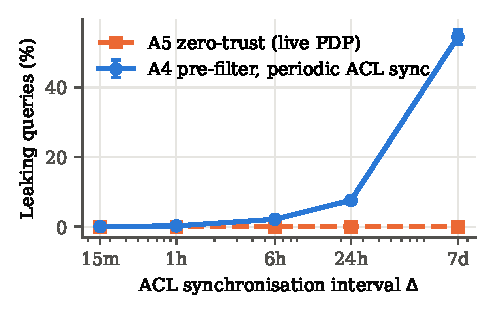
\includegraphics[width=\linewidth]{figs/revocation.pdf}
\caption{E2: post-revocation queries that leak versus ACL snapshot sync interval.}
\label{fig:rev}
\end{minipage}\hfill
\begin{minipage}[t]{0.48\linewidth}\centering
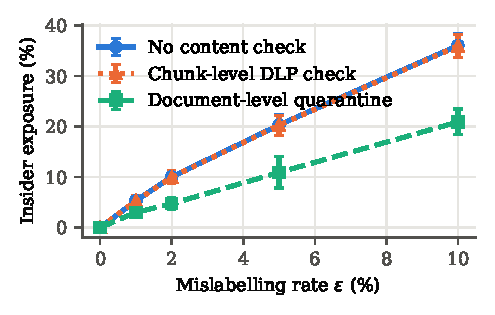
\includegraphics[width=\linewidth]{figs/labelnoise.pdf}
\caption{E5: insider exposure versus mislabelling rate.}
\label{fig:noise}
\end{minipage}
\end{figure}

\begin{figure}[t]
\centering
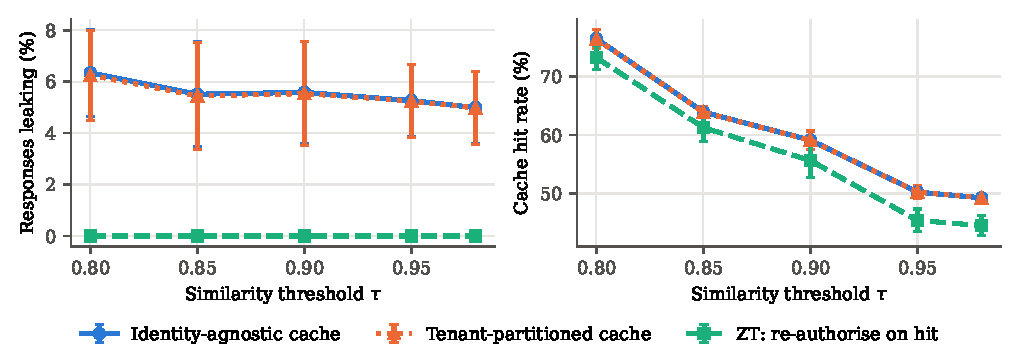
\includegraphics[width=0.82\linewidth]{figs/cache.pdf}
\caption{E3: semantic-cache leakage (left) and hit rate (right) versus similarity threshold.}
\label{fig:cache}
\end{figure}

\section{Results II: In-Flight Revocation and the Release Gate}
\label{sec:resB}

\begin{table}[t]
\centering
\caption{E6: release-stage strategies under departing-insider revocations (200 events per seed, 5 seeds; mean \pmci{95\% CI}). Replica lag mean 2\,s; post-processing gap median 0.3\,s. Overhead is latency added by the release decision.}
\label{tab:inflight}
\small
\setlength{\tabcolsep}{3.5pt}
\begin{tabular}{l|ccc|ccc|c}
\toprule
& \multicolumn{3}{c|}{Chat (median 4\,s)} & \multicolumn{3}{c|}{Agentic (median 60\,s, 3 hops)} & Overhead\\
Strategy & Unsafe/rev. & $P$(any) & Window (s) & Unsafe/rev. & $P$(any) & Window (s) & p50 / p95 (ms)\\
\midrule
S0 Retrieval, TTL 5\,min & 3.09\pmci{0.20} & 81.1\% & 113 & 1.91\pmci{0.14} & 91.4\% & 167 & 0 / 0\\
S1 Retrieval, live & 0.143\pmci{0.020} & 14.1\% & 0.6 & 0.644\pmci{0.013} & 64.4\% & 37.7 & 0 / 0\\
S2 + non-atomic recheck & 0.050\pmci{0.013} & 5.0\% & 0.1 & 0.025\pmci{0.012} & 2.5\% & 0.1 & 10 / 23\\
S3 + atomic gate, replica & 0.047\pmci{0.016} & 4.7\% & 0.1 & 0.024\pmci{0.016} & 2.4\% & 0.1 & 10 / 23\\
S4 + fenced gate, authority & \textbf{0.000} & \textbf{0.0\%} & 0.0 & \textbf{0.000} & \textbf{0.0\%} & 0.0 & 40 / 91\\
\bottomrule
\end{tabular}
\end{table}

\paragraph{Retrieval-time authorisation alone does not survive revocation (RQ3).}
\Cref{tab:inflight} shows that with a 5-minute entitlement cache (S0), 81\% of chat revocations and 91\% of agentic revocations are followed by at least one unsafe release. On average there are 3.1 and 1.9 unsafe releases respectively, spread over roughly two to three minutes. The TTL is in effect the revocation service level (\cref{fig:ttl}). At a 1-hour TTL a chat-style insider receives 36.5 unsafe responses per revocation. Making the retrieval-time check live (S1) helps chat, where requests are short, but not agentic work. A 60-second, three-hop task that retrieved evidence before the revocation releases it afterwards in 64.4\% of events, with a mean exposure window of 37.7\,s. \emph{The longer the request, the less retrieval-time authorisation means.}

\begin{figure}[t]
\centering
\begin{minipage}[t]{0.48\linewidth}\centering
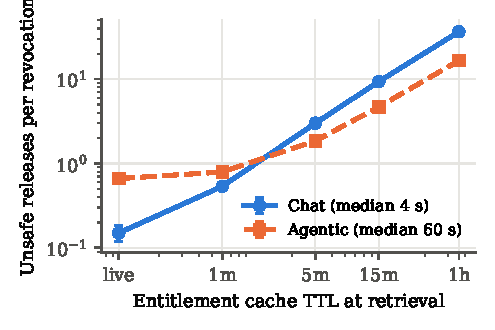
\includegraphics[width=\linewidth]{figs/ttl.pdf}
\caption{E6: unsafe releases per revocation versus entitlement-cache TTL at retrieval (S0, no release gate). Log--log axes.}
\label{fig:ttl}
\end{minipage}\hfill
\begin{minipage}[t]{0.48\linewidth}\centering
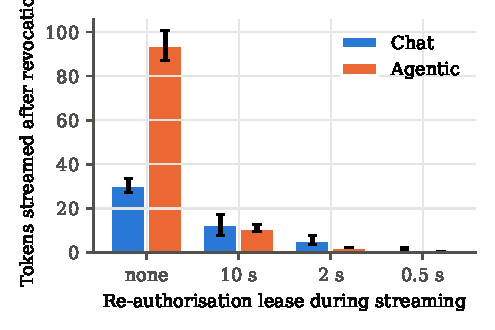
\includegraphics[width=\linewidth]{figs/stream.pdf}
\caption{E7: tokens streamed after revocation per revocation event, by re-authorisation lease interval (300-token responses).}
\label{fig:stream}
\end{minipage}
\end{figure}

\paragraph{A recheck is necessary but not sufficient, and atomicity alone buys nothing.}
Adding a release-time recheck (S2) cuts unsafe releases by 65\% for chat and 96\% for agentic work relative to S1. The residual comes from two gaps: post-processing between the check and the commit, and the staleness of the replica the check reads. Making the gate atomic while still reading the replica (S3) gives no measurable improvement at the default 2\,s lag (0.047 vs.\ 0.050 chat; 0.024 vs.\ 0.025 agentic). \Cref{fig:lag} explains why. The two gaps add up, and the replica lag dominates the sub-second post-processing gap. At zero lag, atomicity matters: S3 reaches 0 while S2 still leaks 0.011 (chat) and 0.004 (agentic). At 30\,s lag, S2 and S3 are indistinguishable (0.371 vs.\ 0.363 for chat). Increasing the post-processing gap from 0.05\,s to 3\,s raises S2's chat leakage from 0.032 to 0.104. Only the fenced gate on the authority (S4) is zero at every lag and gap we tested. It costs one authority round trip, 40\,ms at the median and 91\,ms at p95 under our assumed latencies, which is small next to multi-second generation. \emph{Atomicity and freshness are jointly necessary; neither is sufficient alone.} This is the empirical counterpart of assumptions (C4) and (C5).

\begin{figure}[t]
\centering
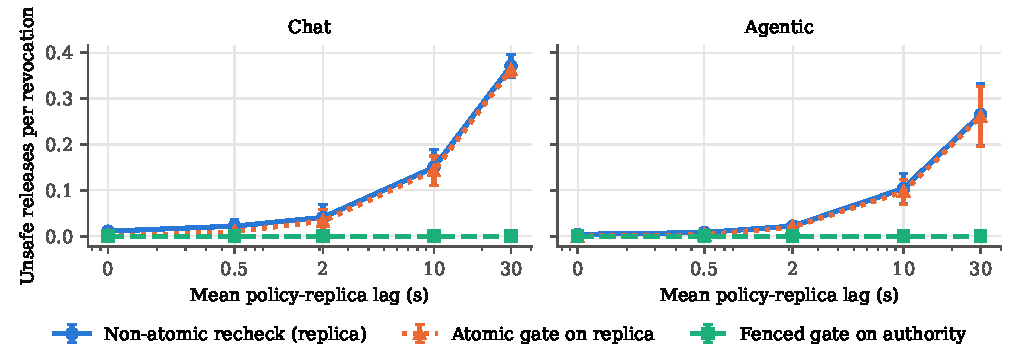
\includegraphics[width=0.85\linewidth]{figs/lag.pdf}
\caption{E6: unsafe releases per revocation versus mean policy-replica lag. The atomic gate on a replica (S3) tracks the non-atomic recheck (S2) once lag exceeds the post-processing gap; only the fenced gate on the authority (S4) remains at zero.}
\label{fig:lag}
\end{figure}

\paragraph{Residual risks under the fenced gate (RQ4).}
\Cref{tab:residual} quantifies what happens when assumptions (C1) and (C3) fail, and what the fail-closed behaviour costs.
\begin{itemize}\itemsep0pt
\item \textbf{Provenance gaps (C1):} if each dependency is missing from the provenance record with probability $q{=}25\%$, as can happen with untracked cache hits, agent summaries or tool results, the fenced gate releases 0.021 (chat) and 0.051 (agentic) unsafe responses per revocation. That is about 8\% of S1's agentic level. Multi-hop tasks are more sensitive because they carry more dependencies.
\item \textbf{Streaming (C3):} streaming without re-authorisation emits 30.5 (chat) and 93.9 (agentic) tokens after each revocation (\cref{fig:stream}). Re-authorisation leases trade leakage for check volume. A 2\,s lease reduces leakage to 5.6 and 2.3 tokens at 2.5 and 38.5 checks per request; a 0.5\,s lease gives 1.5 and 0.5 tokens at 8.6 and 153 checks. Only buffering until the commit gives zero, at the price of losing incremental display.
\item \textbf{Availability:} a fail-closed gate falsely blocks requests at the policy service's unavailability rate (0.10\%, 0.49\% and 1.00\% for 99.9/99.5/99\% availability). Because outages last tens of seconds, a 2\,s retry budget barely helps. A 10\,s budget converts roughly a quarter of the blocks into delays averaging 4.8\,s.
\end{itemize}

\begin{table}[t]
\centering
\caption{E7--E9: residual risk and cost of the commit-time gate (mean over 5 seeds).}
\label{tab:residual}
\small
\begin{tabular}{lcc}
\toprule
\multicolumn{3}{l}{\emph{E8 Provenance gaps (S4): unsafe releases per revocation}}\\
Dependency miss rate $q$ & Chat & Agentic\\
\midrule
0\% / 1\% / 5\% & 0.000 / 0.000 / 0.003 & 0.000 / 0.002 / 0.006\\
10\% / 25\% & 0.009 / 0.021 & 0.016 / 0.051\\
\midrule
\multicolumn{3}{l}{\emph{E7 Streaming: tokens after revocation per event (checks per request)}}\\
Lease & Chat & Agentic\\
\midrule
None & 30.5\pmci{3.2} (0) & 93.9\pmci{6.9} (0)\\
10\,s & 12.6\pmci{4.7} (1.0) & 11.1\pmci{1.5} (8.1)\\
2\,s & 5.6\pmci{2.0} (2.5) & 2.3\pmci{0.1} (38.5)\\
0.5\,s & 1.5\pmci{0.7} (8.6) & 0.5\pmci{0.1} (152.6)\\
\midrule
\multicolumn{3}{l}{\emph{E9 Fail-closed gate: false-block rate (retry budget $B$ = 0 / 2 / 10\,s)}}\\
PDP availability & False blocks & Delayed (mean delay)\\
\midrule
99.9\% & 0.100 / 0.093 / 0.072\% & -- / 0.007\% (1.0\,s) / 0.028\% (4.8\,s)\\
99.5\% & 0.488 / 0.456 / 0.352\% & -- / 0.031\% (1.0\,s) / 0.135\% (4.8\,s)\\
99.0\% & 1.004 / 0.942 / 0.722\% & -- / 0.062\% (1.0\,s) / 0.282\% (4.7\,s)\\
\bottomrule
\end{tabular}
\end{table}

\paragraph{Prototype: real interleavings confirm the race (E10).}
\Cref{tab:proto} reports the multithreaded prototype under adversarial revocation pressure: 32 threads, about 4{,}000 revocations per 10-second run and 5 runs per strategy. Retrieval-only authorisation (B0) released a revoked dependency after 85.8 of every 100 revocations. The non-atomic recheck (B1) still released 12.3 per 100, with every unsafe release caused by a revocation that landed between its check and its commit. The fenced commit (P) released 0 unsafe responses across 30{,}814 audited releases, and also 0 across nine further runs with 8, 32 and 128 threads. Its gate latency was indistinguishable from B1's (p50 5.63 vs.\ 5.62\,ms, p95 9.66\,ms in both, dominated by post-processing). Serialising the commit with revocations therefore added no measurable latency at these scales. The prototype's rates reflect a deliberately extreme revocation schedule and should be read as a stress test of the ordering logic, not as deployment frequencies.

\begin{table}[t]
\centering
\caption{E10: multithreaded prototype (32 threads, 10\,s runs, 5 runs per strategy, mean \pmci{95\% CI}). Unsafe releases are classified by replaying the sequence-ordered authority log.}
\label{tab:proto}
\small
\begin{tabular}{lccccc}
\toprule
Strategy & Releases & Revocations & Unsafe releases & Unsafe / 100 revocations & Gate p50 / p95 (ms)\\
\midrule
B0 Retrieval-only & 9{,}638 & 4{,}089 & 3{,}509\pmci{45} & 85.8\pmci{0.3} & 5.61 / 9.65\\
B1 Non-atomic recheck & 6{,}658 & 4{,}058 & 499\pmci{15} & 12.3\pmci{0.3} & 5.62 / 9.66\\
P Fenced commit & 6{,}163 & 4{,}062 & \textbf{0} & \textbf{0.0} & 5.63 / 9.66\\
\bottomrule
\end{tabular}
\end{table}

\section{Discussion and Recommendations}
\label{sec:discussion}
The measurements separate \emph{whether} access control exists from \emph{when and where it remains correct}. A static evaluation would rank query-time pre-filtering as optimal and declare the problem solved. Each dynamic condition we model breaks that conclusion: sync lag, derived artefacts, caches, mislabelling, long-running requests, replica staleness, streaming and provenance gaps. In every case, the effective remedy is a zero-trust principle applied at the stage where the failure occurs. The measured costs are small: about 0.1\,ms of policy evaluation per query, two points of Hit@5, and one authority round trip per response.

For enterprise RAG deployments, we recommend the following:
\begin{enumerate}\itemsep0pt
\item Propagate the end user's identity to retrieval and never retrieve as a service principal (A0: 94\% benign exposure).
\item Do not rely on tenant partitioning for boundaries inside the organisation (A1: 81\%).
\item Enforce access inside retrieval (pre-filtering), not after it (a 17--34 point Hit@5 gap).
\item Treat every cache and snapshot TTL as a revocation service level. Prefer event-driven revocation, for example CAEP-style push events~\cite{caep2025}, or per-request decisions.
\item Label derived artefacts with the least upper bound of their sources, and re-authorise cached contexts on every hit.
\item Gate the release of every response with a check of its full dependency set against the \emph{authoritative} policy, in the same ordering domain as revocations. A recheck against a replica, atomic or not, leaves a window equal to the replica's lag.
\item Buffer responses until the gate decides. Where streaming is required, use short re-authorisation leases and report the residual leakage explicitly.
\item Track provenance transitively across caches, agent summaries and tool outputs, because the gate is only as complete as $\mathrm{Deps}(o)$.
\item Choose fail-closed or fail-open behaviour per data class, and size retry budgets to the outage distribution, not to typical latency.
\item Invest in labelling quality and ingestion-time consistency checks; mislabelling is the dominant residual risk once enforcement is correct.
\end{enumerate}

\section{Limitations and Threats to Validity}
\label{sec:limits}
\textbf{Synthetic data and parameters.} The corpus and the request-timing distributions are generated, not taken from a deployment. Absolute rates depend on the parameters we assumed: generation time, post-processing gap, replica lag, think time and the share of queries that target lost documents. We sweep the most influential ones and release every parameter so that practitioners can substitute measured values. The relative ordering of strategies and the qualitative interactions, such as atomicity being ineffective without freshness, are the intended findings.

\textbf{No LLM in the loop.} Leakage is measured at the context boundary and at release; the share of exposed content that an attacker can actually extract depends on the model~\cite{zeng2024good,qi2024spill}. Model-level defences are not evaluated.

\textbf{Retrievers.} TF-IDF and LSA stand in for neural embedding models. Both support the same conclusions, but validation on production embeddings and vector databases is needed.

\textbf{Partly by construction.} The zero-trust controls reach zero in the experiments that target their own mechanism. The contribution is to measure the \emph{magnitude} of the alternatives' failures, the \emph{interactions} between mechanisms and the \emph{cost} of the controls, and to measure residual risk when the controls' assumptions are relaxed (E5, E7--E9).

\textbf{Prototype scope.} E10 runs in a single process with a local lock. A distributed deployment must implement the same ordering with a linearisable store, for example version-fenced compare-and-set on the policy record or short-lived signed release capabilities. It will add network round trips that we model but did not measure.

\textbf{Literature coverage.} Our review is targeted rather than systematic, and we make no claim that the individual mechanisms (rechecks, fencing, provenance, fail-closed gates) are new. The contribution is their joint evaluation across the RAG lifecycle.

\section{Conclusion}
Authorisation in enterprise RAG is not a retrieval-time event but a property of the whole request lifecycle. Shared and tenant-partitioned indexes expose unauthorised content to most benign queries. Pre-filtering is optimal only while entitlements, labels and caches stay in sync. Under revocation, retrieval-time checks leak for as long as entitlements are cached and as long as requests run. A release-time recheck is necessary but not sufficient: it must be both atomic with the commit and fresh with respect to the authoritative policy. A fenced commit-time gate achieves this at the cost of one round trip. Its remaining risks are streaming, provenance completeness and availability, and we quantify each. Future work will validate these results on production embedding models, LLM serving stacks and distributed policy engines.

\section*{Code and Data Availability}
All code, data generators, raw per-seed results and figure scripts are released with this paper.
% TODO: insert repository URL
The following commands reproduce every reported number on a laptop CPU in about 20 minutes: \texttt{python -m ztrag.experiments}, \texttt{python -m ztrag.inflight} and \texttt{python -m ztrag.proto}.

\section*{Ethics Statement}
All data is synthetic and generated programmatically; no real personal records, employer data or production systems were used. The probes evaluated operate against a simulated system and provide no new offensive capability.

\section*{Use of AI Tools}
% Edit to match your venue's policy and your actual process.
An AI assistant was used to help implement the benchmark and simulation code and to draft and edit the manuscript. The author designed the research question, reviewed all code, verified every reported result against the released outputs and every reference against its source, and takes full responsibility for the content.

\bibliographystyle{plainnat}
\bibliography{refs}
\end{document}
